%----------------------------------------------------------------------------
%----------------------------------------------------------------------------
Suppose the dynamics of some four level quantum system is given by
%----------------------------------------------------------------------------
%----------------------------------------------------------------------------
\begin{equation}
i\frac{\partial}{\partial t} \ket{\Psi}
=
i\left(
\begin{array}{cccc}
0 & \alpha & 0 & 0 \\
-\alpha & 0 & \beta & 0 \\
0 & -\beta & 0 & \gamma \\
0 & 0 & -\gamma & 0 
\end{array}
\right)
\ket{\Psi},
\label{three dynamics}
\end{equation}
%----------------------------------------------------------------------------
where the square of the nth element in $\Psi$ is the probability of finding the system in the nth state, $\alpha$ is the coupling field between the zeroth (ground) and first state, $\beta$ is the coupling field between the first and second state, and $\gamma$ is the coupling field between the second and third state. Using the same methods as in Section \ref{basic_two_level}, it can be shown that closed non-degenerate four level quantum systems with three completely resonant ``ladder'' coupling fields can be described this way in the energy basis (see figure \ref{three color ladder}).
%----------------------------------------------------------------------------
%----------------------------------------------------------------------------
% 3_color_ladder.tex
% by Troy Hix, April 2005
%----------------------------------------------------------------------------
%----------------------------------------------------------------------------
\begin{figure}
\setlength{\unitlength}{2cm}
\begin{center}
\begin{picture}(3.3,3.2)
\linethickness{1mm}
\put(0,3.0){\line(1,0){3}}
\put(0,2.0){\line(1,0){3}}
\put(0,0.8){\line(1,0){3}}
\put(0,0.0){\line(1,0){3}}
\put(3.1,3.0){$\ket{3}$}
\put(3.1,2.0){$\ket{2}$}
\put(3.1,0.8){$\ket{1}$}
\put(3.1,0.0){$\ket{0}$}
\thinlines
\put(1.0,2.0){\vector(0,1){0.98}}
\put(1.0,0.8){\vector(0,1){1.18}}
\put(1.0,0.0){\vector(0,1){0.78}}
\put(1.2,2.5){$\gamma$}
\put(1.2,1.4){$\beta$}
\put(1.2,0.4){$\alpha$}
\end{picture}
\end{center}
\caption[Four level, three field diagram]{Four level, three field diagram. Ground state $\ket{0}$, first excited state $\ket{1}$, second excited state $\ket{2}$ and third excited state $\ket{3}$ are coupled by fields $\alpha$, $\beta$, and $\gamma$ so that population transfers from the ground state to the third excited state}
\label{three color ladder}
\end{figure}
%----------------------------------------------------------------------------
%----------------------------------------------------------------------------

%----------------------------------------------------------------------------
%----------------------------------------------------------------------------
%----------------------------------------------------------------------------
%----------------------------------------------------------------------------
Again we consider temporally localized coupling fields of the form (\ref{gaussian}). Let the positions of $\alpha$ and $\gamma$ be given in terms of $\beta$'s position; namely let $\Delta_\alpha$ be the temporal distance alpha \emph{leads} beta and $\Delta_\gamma$ be the temporal distance gamma \emph{lags} beta; specifically
%----------------------------------------------------------------------------
\begin{subequations}
\begin{eqnarray} 
t_\alpha & = & t_0 - \Delta_\alpha \\
t_\beta  & = & t_0 \\
t_\gamma  & = & t_0 + \Delta_\gamma
\end{eqnarray}
\label{xxx}
\end{subequations}
%----------------------------------------------------------------------------
where $t_0$ is the middle of the pulse sequence (and the position of $\beta$). Thus, for a sequential order as shown in Figure \ref{three pulses}, both $\Delta_\alpha$ and $\Delta_\gamma$ are positive.
%----------------------------------------------------------------------------
%----------------------------------------------------------------------------
% 3_pulses.tex
% by Troy Hix, March 2005
%----------------------------------------------------------------------------
\begin{figure}
\centering
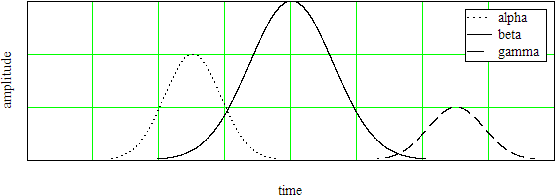
\includegraphics[width=5.00in]
{3_pulses/3_pulses.png}\\
\caption[Three pulse sequence example]{Three pulse sequence example. In general the pulses $\alpha$, $\beta$, and $\gamma$ have arbitrary widths $\sigma_\alpha$, $\sigma_\beta$, and $\sigma_\gamma$ as well as arbitrary amplitudes $A$, $B$, and $C$.}
\label{three pulses}
\end{figure} 
%----------------------------------------------------------------------------

%----------------------------------------------------------------------------
%----------------------------------------------------------------------------
%----------------------------------------------------------------------------
